\chapter{Working with objects - Generalized image analysis workflows}

In the module 'Measuring Intensities', you explored how you can manually define a region of interest and perform intensity measurements on this region. While this is already a commonly found approach, the manual labor can be very tedious or impossible with given resources. Another aspect that is often neglected is the possible (and likely) introduction of bias - outside actual clinical studies, a double blind approach is very uncommon. This module will present all components of a generalized image analysis workflow:

\begin{enumerate}
	\item Obtain raw image data. In this course, we assume that raw image data already exists and that this image data is suitable for the necessary analysis.
	\item Image visualization and preprocessing. This typically involves simple pixel operations and multiple image filters.
	\item Identify objects of interest (image segmentation). The preprocessed image is used to generate pixel label maps; in a simple case, this is based on a binary image (black = background, white = objects of interest).
	\item Manipulate objects. The detected objects are modified and enhanced. For example, this can involve cleaning object boundaries, removing holes, splitting or merging objects.
	\item Perform measurements. In the last step, you convert the finally identified objects into numbers for further (statistical) analysis. For example, the derived numbers can be based on intensity, shape, texture or object relationships.
\end{enumerate}

\section{Image preprocessing}

We now generalize this concept of pixel operations by looking at an image as a discrete function. For a 2D image, $f(x,y)$ maps from $R^2$ to $R$, giving the intensity at position $(x,y)$. In this view, any pixel operation $o$ can be expressed as $g\left(x,y\right)=o\left(f\left(x,y\right)\right)$, where $g(x,y)$ is the modified image. The operations we already know are either simple arithmetic- or histogram-based methods. 

Another type of very powerful operations is the \emph{image filter}. Often, image preprocessing involves the (sequential) application of various image filters. Image filters are local operations where the \emph{neighborhood} (surrounding pixels) of each pixel determines the new intensity value. The pixel neighborhood is also called the \emph{kernel}. These filters are mainly used to smooth the image (suppress high frequencies) or enhance edges (suppress low frequencies).

Image filters can be performed on the spatial domain (the image you know with x/y/z axes) or on the frequency domain (Fourier transformed image). For simplicity, we completely skip the Fourier transform, frequency domain filtering and the mathematical reasoning why it can make sense to transform an image into the frequency domain, perform (linear) filtering, and transform the image back to the spatial domain. Furthermore, we will restrict our explanations and examples to 2 dimensional (discrete) images. 

\subsection{Convolution, Correlation \& Kernels}

Convolution is the mathematical operation behind many of the image filters we will discuss. As described, the basic idea is that a neighborhood of pixels, a window with finite size and shape, is placed on top of each pixel and that the new pixel value is determined by the weighted sum of all pixels within this neighborhood. This window with the weights is called the \emph{kernel}. 

Again, we look at the image as a matrix of pixels and do the same for the kernel, the neighborhood with the weights. We then perform the weighted sum of all pixels within the kernel and repeat for every pixel in our image (Fig. \ref{fig:convolution-example}).

\begin{figure}[!ht]
	\centering
		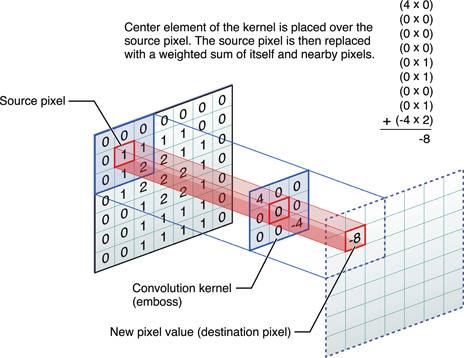
\includegraphics[width=0.70\textwidth]{mod3/figures/convolution-example.png}
	\caption{Convolution example. A single location of a 2D convolution is shown. The image was taken from \cite{MacDev2011}}
	\label{fig:convolution-example}
\end{figure}

If we want to convolve a pixel at position $(x,y)$ of an image $F$ with the rectangular kernel $K$, centered around $(x,y)$, with width $\omega$, we can write:
\[
	\left[F\ast K\right]\left(x,y\right)=\sum_{i=-\omega}^{i=\omega}\sum_{j=-\omega}^{j=\omega}K\left(i,j\right)\cdot F\left(x-i,y-j\right)
\]

For better illustration, let us perform the convolution on a small example, we average an image showing a vertical white line on black background with a 3x3 smoothing kernel (this operation is explained below):
\[
	\begin{array}{|c|c|c|c|c|}
	\hline
	0&0&255&0&0\\
\hline
0&0&255&0&0\\
\hline
0&0&255&0&0\\
\hline
0&0&255&0&0\\
\hline
0&0&255&0&0\\
\hline
	\end{array} 
	\ast 
	\begin{array}{|c|c|c|}
	\hline
	1/9&1/9&1/9\\
\hline
1/9&1/9&1/9\\
\hline
1/9&1/9&1/9\\
\hline
	\end{array}
	=
	\begin{array}{|c|c|c|c|c|}
	\hline
	0&57&57&57&0\\
\hline
0&85&85&85&0\\
\hline
0&85&85&85&0\\
\hline
0&85&85&85&0\\
\hline
0&57&57&57&0\\
\hline
	\end{array} 
\]

Figure \ref{fig:convolution-demo} looks at a few steps of the convolution to illustrate how the resulting image is calculated.

\begin{figure}[!ht]
	\centering
		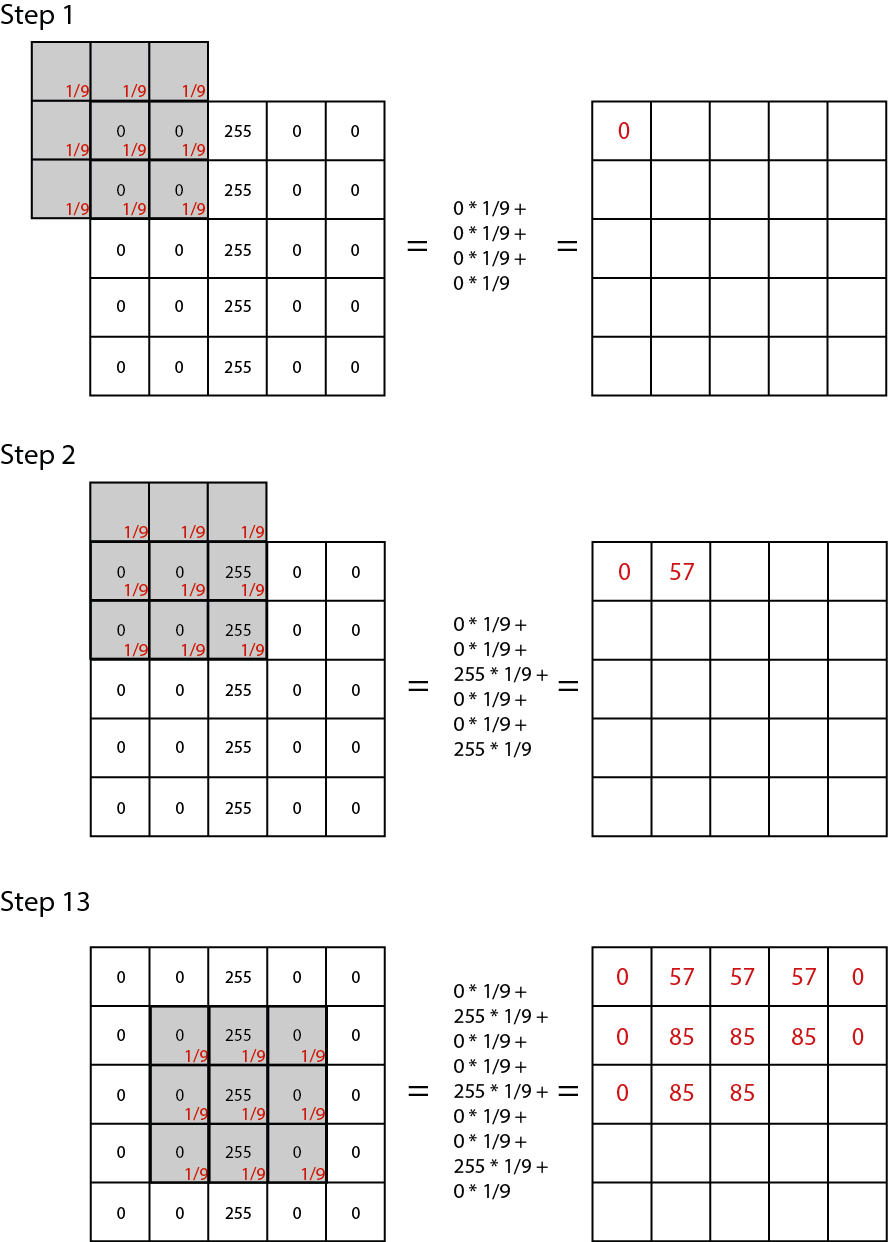
\includegraphics[width=0.60\textwidth]{mod3/figures/convolution-demo.png}
	\caption{Example steps of the convolution}
	\label{fig:convolution-demo}
\end{figure}

\newpage
\begin{taskbox}{Working with Image Filters}
Let us compare the previous example with the operation performed in Fiji.

\begin{enumerate}
	\item Generate an 8-bit, 5x5 pixel black image with a white vertical line as shown in the convolution example. Duplicate and zoom in to observe individual pixels and check whether the intensity values of the black pixels are zero and the values of the white pixels are 255.
	\item Go to \texttt{[Process > Filters > Convolve...]}. Change the default kernel in the Convolver dialog to (Fig. \ref{fig:convolver-dialog}): 
	\[
		\begin{array}{|c|c|c|}
	\hline
	1&1&1\\
\hline
1&1&1\\
\hline
1&1&1\\
\hline
	\end{array}
\]
	Note that we did not enter 1/9; the values are automatically divided by the number of elements in the kernel if 'Normalize Kernel' is ticked. Select 'Preview' if you directly want to observe the effects of your chosen kernel.
	
	\begin{minipage}[t]{\linewidth}
		\begin{center}
		\adjustbox{valign=t}{%
			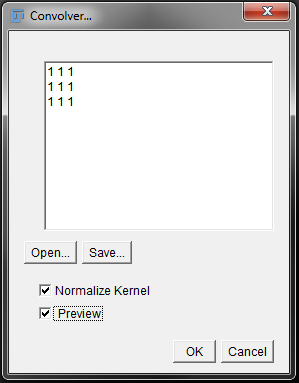
\includegraphics[width=0.3\textwidth]{mod3/figures/convolver-dialog.png}%
		}
		\medskip
		\captionof{figure}{Convolver Dialog.}\label{fig:convolver-dialog}
		\end{center}
	\end{minipage}
	
	\item Compare the new pixel values with the values shown in the example. Do you observe any differences? You should note that pixels at the border of the image can show differences. This is caused by a different way to treat image borders. While the example simply ignores kernel positions outside the image, Fiji increases the image size to fit the kernel within the image (padding). These extra pixels are duplicates of border pixels and therefore, the results differ.
	
	\end{enumerate}
\end{taskbox}

\minisec{Convolution and Correlation}

A convolution is a correlation with the kernel rotated by 180 degrees. This makes no difference if the filter is symmetric (e.g. Gaussian). The reflection of the kernel has a few important effects. One is that the convolution is associative ($f * g * h = f * (g * h)$) while the correlation is not; i.e. the associativity allows you to pre-convolve several filters into a single filter that gets applied to your image. The correlation describes the comparison between the kernel and the pixel neighborhood and is, for example, used in template matching as associativity is not important for this task. Also, the convolution is a multiplication in the frequency domain and it can be faster to perform the filtering in the frequency domain (depending on image and kernel size). 

\begin{taskbox}{The point spread function (PSF)}

The image you obtain with a microscope is blurred by the optics of the microscope itself. The point spread  function describes the impulse response of the microscope, i.e. the 3D diffraction pattern resulting from a single point. In microscopes (non-coherent systems), the image formation process is linear, which means that the imaging of many objects produces a result that is the sum of individually imaged objects. Therefore, image formation in a microscope can be seen as a convolution of the true object with the PSF. Estimating the PSF of a microscope then allows image deconvolution -- a process where the true image is estimated by trying to reverse the effects of the convolution. The problem is that deconvolution is an ill-posed problem -- no solution, or no unique solution might exist and noise can strongly influence a solution. Computing intense deconvolution algorithms are used to approximate the true image; a PSF for deconvolution can be obtained by measuring sub-resolution beads with know radii or by theoretical estimation using parameters of the optical system. 

In this exercise, we use an artificial ground-truth image and convolve this image with a single slice of a cropped and low bit-depth version of a measured PSF. 

\begin{enumerate}
	\item Open the images artificial-groundtruth.tif and PSF-LeicaSP8-63x-Ar488.tif in /mod3/data. The image shows a cropped, 8 bit, x/y slice through a 3D PSF taken at the center (focal plane). 
	\item Convolve the groundtruth image with the PSF by loading the file PSF-LeicaSP8-63x-Ar488.txt in the convolver dialog.
	\item Compare the groundtruth image with the convolved image. This is what happens every time you take an image with the microscope! (Although this is only a 2D, simplified example).
	\end{enumerate}
\end{taskbox}

\subsection{Linear Filters}
Convolution is the mathematical operation behind linear filters; and in the following, we will look at some of the most common linear filters available.

\subsubsection{Averaging filter}
An averaging operation (also called smoothing, arithmetic mean or box-car filter) is used to suppress noise in an image. The size of the structures that are suppressed is dependent of the kernel size. Small fluorescence fluctuations will be suppressed by a small filter; increasing the filter size, larger structures will be reduced in size and smoothed into the surrounding regions. Manually varying the filter size allows you to decide the optimal scale of the smoothing for your analysis.

This filter was already shown in the convolution demonstration and the first exercise, the kernel (without normalization to the number of elements) is:
	\[
		\begin{array}{|c|c|c|}
	\hline
	1&1&1\\
\hline
1&1&1\\
\hline
1&1&1\\
\hline
	\end{array}
\]

\begin{taskbox}{Averaging images}

\begin{enumerate}
	\item Open the image microtubuli.tif in /mod3/data. Zoom into the image and observe the fluorescence fluctuations along the microtubuli.
	\item Preview the smoothing filter with a kernel size of 3x3 (see above), using \texttt{[Process > Filters > Convolve...]}. Then increase the kernel size to 5x5 and 7x7 and compare the results (duplicate the images!). What happens when the size of the kernel becomes larger? Can you enter a kernel size of 2x2?
	\item The averaging filter has its own direct command in Fiji. Go to \texttt{[Process > Filters > Mean...]}. You can choose a radius and optional preview in the next window. A radius can be given instead of size in X and Y as the kernel mask is circular -- the neighborhood can be defined arbitrarily! Circular kernels are common as pixels the outermost pixels have the same distance to the pixel of interest (Circular kernels can be shown with \texttt{[Process > Filters > Show Circular Masks...]}). Try different radii to obtain the best smoothing to suppress small fluorescence fluctuations.
	\item To show the effect of the filter more directly, you can subtract the smoothed from the original image.
	\end{enumerate}
\end{taskbox}

\subsection{Gradient filters}

Image features with high spatial frequencies (edges) are those where intensity varies greatly over short image distances (e.g. neighboring pixels). These changes over distance can be seen as a derivative (like velocity is the derivative of position over time). For our images, we use the \emph{gradient} as a generalization of the derivative of a function in one dimension (like velocity), to a function in several dimensions (like our 2D images). For our 2D images $I(x,y)$, we can write the gradient as:
\[
	\nabla I(x,y)=\left(\frac{\delta I}{\delta x},\frac{\delta I}{\delta y}\right)
\]

A common use for gradient filters is edge detection. A large gradient value of a pixel might indicate an edge and edges could then be traced along those pixels (perpendicular to gradient direction). For example, edge detection can be very useful if your structures of interest vary in absolute intensity but are always distinctive against their direct surroundings. 

\minisec{Find Edge (Sobel Filter)}
The find edge filter is used to create an image which emphasizes edges. It uses an approximation of the gradient to create two 3x3 kernels which are convolved with the original image $I$ (kernels are an approximation of the derivative in horizontal, respective vertical direction) to create two output images $J_{x}, J_{y}$:
	\[
		J_{x}=\left[\begin{array}{ccc}
	1&0&-1\\
2&0&-2\\
1&0&-1\\
	\end{array}\right]\ast I, J_{y}=\left[\begin{array}{ccc}
	1&2&1\\
0&0&0\\
-1&-2&-1\\
	\end{array}\right]\ast I
\]

The gradient magnitude image $J$ is then calculated with:
\[
	J=\sqrt{J_{x}^{2}+J_{y}^{2}}
\]

\minisec{Sharpen (Laplacian Filter)}

The sharpen filter is also often used to emphasize changes in pixel intensities. In this case, the 3x3 kernel is approximated by the sum of the second derivatives:
	\[
		\begin{array}{|c|c|c|}
	\hline
	-1&-1&-1\\
\hline
-1&12&-1\\
\hline
-1&-1&-1\\
\hline
	\end{array}
\]

\begin{taskbox}{Gradient Filters}
\begin{enumerate}
	\item Open the image microtubuli.tif in /mod3/data. Zoom into the image and observe the fluorescence fluctuations along the microtubuli. Remember to duplicate the images before testing any processing.
	\item At first, test the sharpen filter with \texttt{[Process > Sharpen]} and optionally using the kernel in the convolution dialog.
	\item The find edge filter can be tested directly using \texttt{[Process > Find Edges]}. If you want to explore the filter a bit more, you can also generate both filtered images, convert those to 32 bit and perform the calculations by yourself. Are the results identical?
	\item What happens to the noise if you use the sharpen filter? 
	\item What happens if you first use a smoothing filter and then the edge detection filter?
	\end{enumerate}
\end{taskbox}

\subsubsection{Gaussian filters}

A very important linear filter that smooths an image and reduces noise is the \emph{gaussian filter}. In difference to the mean filter, pixels in the neighborhood are weighted with their distance to the pixel of interest. The weights are obtained by a gaussian function where the width $\sigma$ of the gaussian function $g(x,y)$determines the kernel size. $A$ is a scaling factor used for normalization:
\[
	g(x,y)=A e^{\left(\frac{x^2+y^2}{2\sigma^2}\right)}
\]

If you want to smooth your image, it is always a good idea to not only explore the averaging filter but also the gaussian filter. Again, varying $\sigma$, you can determine the optimal filter size for your application.

\minisec{Difference of Gaussian filter (DoG)}
Let's say you want to suppress small structures but also large structures and focus on detecting structures within a certain size range. In this case, you could combine two gaussian filters: one with a small $\sigma$ to suppress small structures and one with a large $\sigma$ to suppress large structures as well. When you then subtract the second filtered image from the first filtered image, the image that is left contains information between both smoothing scales. 

\begin{taskbox}{Gaussian Filters}
\begin{enumerate}
	\item Open the image microtubuli.tif in /mod3/data. Zoom into the image and observe the fluorescence fluctuations along the microtubuli. Remember to duplicate the images before testing any processing.
	\item The gaussian filter can be tested using \texttt{[Process > Filters > Gaussian Blur...]}. 
	\item Try to find an optimal value for $\sigma$.
	\item Implement a DoG filter with $\sigma$ values of $1$ and $10$.
	\end{enumerate}
\end{taskbox}

\begin{taskbox}{Unsharp Mask Filter}
Let's illustrate the power of combining filters and image math with another example. In this case, we will replicate the unsharp mask filter. This is a very common filter available in many software packages, e.g. for photo editing, but has to be used very carefully for quantitative scientific analysis.

\begin{enumerate}
	\item Open the image microtubuli.tif in /mod3/data. Duplicate.
	\item Use a gaussian filter with a $\sigma$ of $2$. 
	\item Multiply the gaussian filtered image with a weight $w$ of $0.8$.
	\item Subtract the weighted image from the original image.
	\item Divide the resulting image by $0.2$. 
	\item Last, compare your results to the results of \texttt{[Process > Filters > Unsharp Mask...]}.
	\end{enumerate}
\end{taskbox}

\subsection{Nonlinear Filters}
In addition to linear filters which can be implemented with a convolution, we can also use nonlinear filters to enhance our images. We will discuss one particular class of such filters (rank filters), focusing on the median filter. This filter or its variants can be very powerful when you want to remove noise but maintain other details of the image or you want to be less susceptible to outliers. 

\minisec{Median, maximum and minimum filters}
For the median, maximum and minimum filters, pixels in the neighborhood are sampled and then sorted by their intensity values. Let's assume you have an 3x3 image part surrounding the pixel with value 100, such as:
	\[
		\begin{array}{|c|c|c|}
	\hline
	0&95&105\\
\hline
0&100&110\\
\hline
0&0&90\\
\hline
	\end{array}
\]
 The sorted list would look like: $0,0,0,0,90,95,100,105,110$. The median filter would update the pixel value from 100 to 90. The mean filter would update to a value of 56. If this pixel is part of an edge, the median filter would be better to maintain this edge. The maximum and minimum filters use the same sorted list but update the pixel with either the highest or the lowest value.

\begin{taskbox}{Median Filter}
\begin{enumerate}
	\item Open the image microtubuli.tif in /mod3/data. Before we do any further processing, we add some Salt-and-Pepper noise using \texttt{[Process > Noise > Salt and Pepper]}. This sets random pixels to the lowest or highest values.
	\item Duplicate the image with added noise and perform the mean filter to suppress the just added noise (find a suitable radius).
	\item Now, use the median filter \texttt{[Process > Filters > Median]} with the same radius.
	\item Which filter works better?
	\end{enumerate}
\end{taskbox}

\begin{taskbox}{Background subtraction and batch processing}
To make this exercise more interesting, we first establish the method we want to use and then apply it to many files automatically. If a certain task is performed multiple times, it is called \emph{batch processing}. 

\begin{enumerate}
	\item Open the image xu2015-adipocytes.tif in /mod3/data. This image was provided as an example image by Elaine Xu (March 2015, Bruening lab, MPI Stoffwechselforschung). The image shows adipocytes and is a good example to illustrate uneven illumination and how to improve the image with background subtraction.
	\item At first, we explore a method to subtract the background. For this, we first perform a Gaussian blur on a duplicate image with a large $\sigma$ of $20$. This creates a very blurry image that already shows that we picked up the uneven illumination. You can look at a line profile in the original and the blurred image.
	\item Now we subtract the original image from the blurred image. Adjust brightness/contrast to confirm that background was subtracted. As the gaussian blur is a lowpass-filter, the subtraction of this lowpass image can be considered as a (pseudo) highpass filtering.
	\item Fortunately, Fiji already has a function embedded that performs a similar operation for background subtraction, called a rolling ball background subtraction (Same idea: somehow calculate an average for every pixel. However, the actual calculations differ). 
	\item We now want to perform the background subtraction on all image files in a certain folder. For this, we \emph{record} our actions and then use the recorded sequence on each of those files.
	\item Close all images except the original xu2015-adipocytes.tif.
	\item To start the recording, perform \texttt{[Plugins > Macros > Record...]}. A Recorder window pops up (Fig. \ref{fig:recorder-dialog}). Make sure that 'Macro' is selected in Record and nothing else.
	
	\begin{minipage}[t]{\linewidth}
		\begin{center}
		\adjustbox{valign=t}{%
			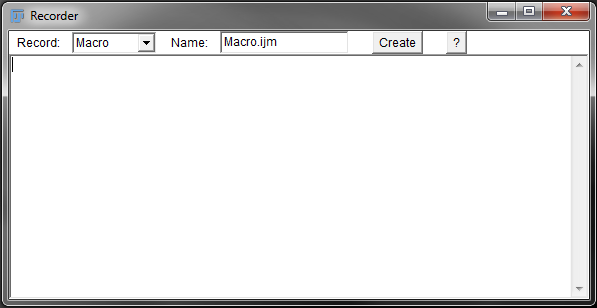
\includegraphics[width=0.8\textwidth]{mod3/figures/recorder-dialog.png}%
		}
		\medskip
		\captionof{figure}{Recorder window.}\label{fig:recorder-dialog}
		\end{center}
	\end{minipage}
	
	\item Do \texttt{[Process > Subtract Background...]}, set the rolling ball radius to $20$ (Fig. \ref{fig:rollingball-dialog}). After you clicked on 'ok', the operation gets performed and the recorder should show following line: \texttt{run("Subtract Background...", "rolling=20");}. 
	
	\begin{minipage}[t]{\linewidth}
		\begin{center}
		\adjustbox{valign=t}{%
			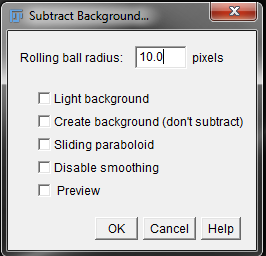
\includegraphics[width=0.3\textwidth]{mod3/figures/rollingball-dialog.png}%
		}
		\medskip
		\captionof{figure}{Subtract background window.}\label{fig:rollingball-dialog}
		\end{center}
	\end{minipage}
	
	\item Select the line and copy (Strg+C). Go to \texttt{[Process > Batch > Macro...]}. In the batch processing window, select the input folder /batch-files in /mod3/data. This folder contains 5 identical adipocyte images with different names. Also, choose an output folder, make sure that this output folder exists. Paste the line of code into the window (Fig. \ref{fig:batch-process-dialog}). and click on 'Process'. Check the chosen output folder for the results. 
	
		\begin{minipage}[t]{\linewidth}
		\begin{center}
		\adjustbox{valign=t}{%
			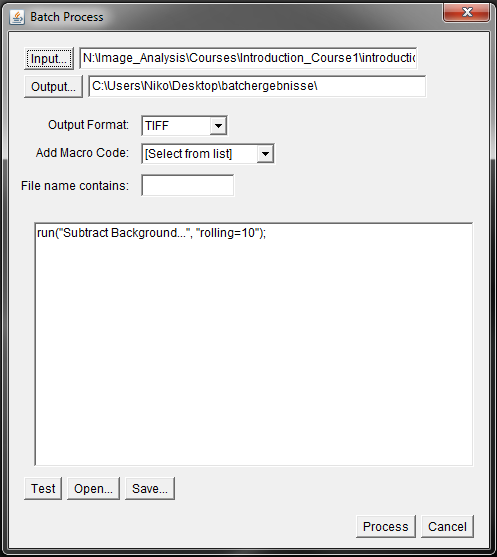
\includegraphics[width=0.8\textwidth]{mod3/figures/batch-process-dialog.png}%
		}
		\medskip
		\captionof{figure}{Subtract background window.}\label{fig:batch-process-dialog}
		\end{center}
	\end{minipage}
	
	\end{enumerate}
\end{taskbox}

When you try to perform a batch processing where a function requires explicit file names the batch processor will fail because it does not know that these need to be replaced (e.g. when the sequence Duplicate Image, Gaussian, Image Calculator is used). In this case, we have to create a macro where individual file names get replaced. Unfortunately, this requires a little bit of very basic understanding of programming principles (we need variables, for-loop and a function). As this is outside the scope of this module, we will not discuss those concepts (however, they are important for more complex automated workflows). 

\section{Image segmentation}

Image segmentation is a process where every pixel in an image obtains a label, such that pixels with the same label share characteristics. Typically, this is done to detect \emph{objects} or structures of interest. Sometimes, these objects are called \emph{connected components}. Basically, this is what you have already done using regions of interest to mark the pixels belonging to a nucleus or cytoplasm. This can be called manual segmentation and works if there is not too much data to analyze. Overall, it is preferable to automate the process of segmentation; not only because it is faster, but also because it should lead to better reproducibility and lower bias of the results. 

\subsection{Thresholding}

A very simple and easy to understand image segmentation method is called \emph{thresholding}. In this method, each pixel belongs to one of two groups: background or foreground (black or white, object or not object). For images obtained with fluorescence microscopy, this is easy to understand: we typically have dark background with light objects. Thresholding image $f\left(x,y\right)$ with a thresholt $T$ then leads to extraction of the objects in image $g\left(x,y\right)$:
	\[
		g\left(x,y\right)=\begin{cases}
		1 &\text{if } f\left(x,y\right)>T\\
		0 &\text{otherwise}
			\end{cases}
\]

Image $g\left(x,y\right)$ is a binary image, only consisting of black and white pixels.

\begin{taskbox}{Thresholding with contrast adjustment}
Let us first have a look at the effects of thresholding using brightness/contrast adjustments.

\begin{enumerate}
	\item Open the image cell-colony.tif in /mod3/data. Open the brightness/contrast adjustment window. Observe the slope of the line that shows the change in (displayed) intensity between the minimum and maximum pixel values in the histogram (Fig. \ref{fig:bc-window}, red line).
	
	\begin{minipage}[t]{\linewidth}
		\begin{center}
		\adjustbox{valign=t}{%
			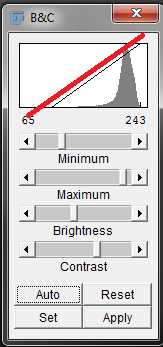
\includegraphics[width=0.3\textwidth]{mod3/figures/bc-window1.png}%
		}
		\medskip
		\captionof{figure}{Brightness and Contrast adjustment.}\label{fig:bc-window}
		\end{center}
	\end{minipage}
	
	\item Now, set the contrast to the maximum value and observe that the slope of the line changes until the line appears nearly vertical. The image is a black and white image now, everything to the left of the line is black, everything right of the line is white (the majority of the pixels as seen in the histogram).
	\item If you now change the brightness, you can move this vertical line around and observe that the number of pixels identified as white (black) changes.
	\end{enumerate}
\end{taskbox}

\begin{taskbox}{Manual thresholding}
Instead of adjusting the contrast, Fiji has a specialized function to adjust the threshold \texttt{[Image > Adjust > Threshold...]}.

\begin{enumerate}
	\item Open the image cell-colony.tif in /mod3/data if it is not already open. 
	\item Do \texttt{[Image > Adjust > Threshold...]} to open the threshold adjustment window (Fig. \ref{fig:adjust-threshold-dialog}). In this window, you can set the intensity for the threshold. Furthermore, you can select whether you have a dark or light background to determine whether you are interested in light or dark objects. Note that you can select a window for your threshold, by setting the lower and upper values to a value outside the extremes. This is called a \emph{density slice} and can be used to detect objects that fall within a certain intensity range.
	
	\begin{minipage}[t]{\linewidth}
		\begin{center}
		\adjustbox{valign=t}{%
			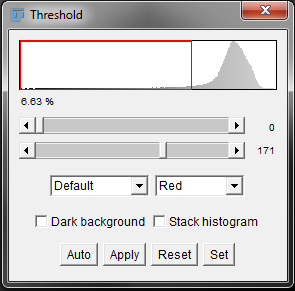
\includegraphics[width=0.4\textwidth]{mod3/figures/adjust-threshold-dialog.png}%
		}
		\medskip
		\captionof{figure}{Adjust threshold window.}\label{fig:adjust-threshold-dialog}
		\end{center}
	\end{minipage}
	
	\item Change values and play with different settings until you think you found an optimal threshold. How difficult is it to obtain an optimal threshold, i.e. how sensitive is the result to your chosen value?
	\end{enumerate}
\end{taskbox}

Manually thresholding an image is already a powerful way to detect objects of interest. But what should you do if you cannot apply the same threshold value for all images you want to analyze? Of course you could manually choose a value for each image. However, this can introduce a bias into your results. A better option would be to automatically determine the optimal threshold value for each image, using the same algorithm. Fiji already has a variety of algorithms that you can choose from (Fig. \ref{fig:all-thresholds}):

\begin{itemize}
	\item Huang
	\item Intermodes
	\item IsoData
	\item Li
	\item MaxEntropy
	\item Mean
	\item MinError
	\item Minimum
	\item Moments
	\item Otsu
	\item Percentile
	\item RenyiEntropy
	\item Shanbag
	\item Triangle
	\item Yen
\end{itemize}

\begin{figure}[!ht]
	\centering
		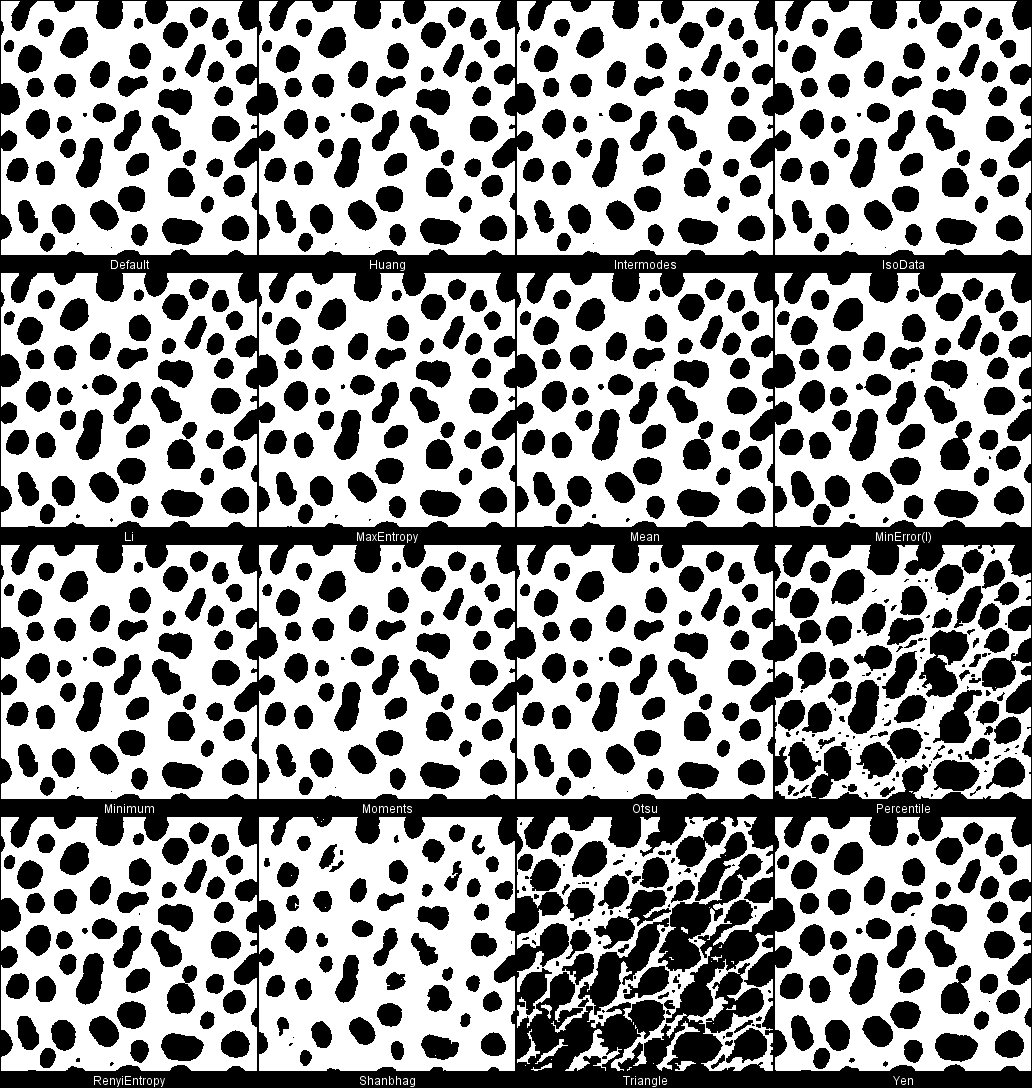
\includegraphics[width=0.80\textwidth]{mod3/figures/all-thresholds.png}
	\caption{Results of all available thresholding methods, using [Image > Adjust > Auto Threshold], Try All. }
	\label{fig:all-thresholds}
\end{figure}

Choosing an algorithm can theoretically be done by looking at the details of the algorithm and determining best which method suits your data. In practice, however, you can simply try all and choose the one that suits your purposes best. 

Let us have a look at one of the thresholding methods, \emph{ Otsu's method}. This algorithm makes the assumption that two classes of pixels are in an image, with each class having a distribution of intensity values. The algorithm calculates the optimum threshold that separates these two classes so that the variance of pixels within each class is minimal. This algorithm is very common, easy to understand and implement. 

\begin{taskbox}{Automated thresholding}
\begin{enumerate}
	\item Open the image hela-cells.tif in /mod3/data. In this task, we first want to automatically identify the nuclei. Select the appropriate channel and duplicate. 
	\item Test all available thresholding methods. You can see that most method already produce very nice results.
	\item In the next step, we want to identify the lysosomes (red). Try to threshold the appropriate channel with Otsu's method. Are the results good enough?
	\item As you can see, the algorithm already works relatively well, but is not good enough for our purposes. Can you think of a reason why the method fails in some parts of the cells? 
	\item After an analysis, we come to the conclusion that background signal is too high in parts of the cell. Therefore, we now first use a background subtraction (e.g. with a rolling ball radius of 10 pixels) before we threshold with Otsu's method. Do the results improve?
	\item Finally,try to use the green channel to identify the cells' cytoplasm. Again, it seems that an image filter might improve the results. Try a gaussian filter with varying sigma values to improve the results. At the end, the result we obtain is not perfect but might be sufficient for our needs. You will see in section about binary images how we could still improve on this thresholding. 
	\end{enumerate}
\end{taskbox}

\subsection{Binary Images}
Thresholding into two pixel classes leads to a binary image. In this section, we will learn how operations on binary images can be used to process an image to facilitate further analysis. 

\subsubsection{Morphological operations}
Morphological operations are very similar to image filters, only that in this case, logical operations are performed on the image. Similar to image filters, a small \emph{structuring element} (kernel in image filters) is moved over the image pixel by pixel and logical operations are performed between the image and the structuring element. In this section, we will discuss the basic morphological operations.

\minisec{Erosion}
Erosion of a binary image $I$ with an structuring element $S$ changes a foreground pixel (white) to background (black) if at least one of the neighbor pixels (defined by $S$) is a background pixel. Erosion is used to shrink or thin an object (foreground) in a binary image; only pixels that were only surrounded by foreground pixels remain (Fig. \ref{fig:morphology-erosion}). In Fiji, the structuring element is a 3x3 pixel square. 

\begin{figure}[!ht]
	\centering
		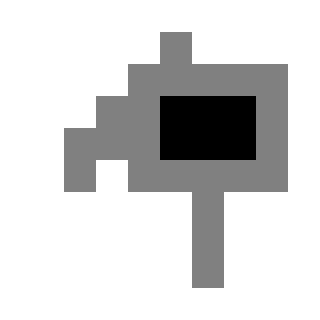
\includegraphics[width=0.40\textwidth]{mod3/figures/morphology-erosion.png}
	\caption{Erosion. Gray pixels indicate the original image. Black pixels remain after erosion with a 3x3 square. For display reasons, black pixels indicate foreground, white pixels background.}
	\label{fig:morphology-erosion}
\end{figure}

\minisec{Dilation}
In contrast to erosion, dilation grows or thickens an object in a binary image. A background pixel is changed to foreground if at least one pixel in the neighborhood is a foreground pixel (Fig. \ref{fig:morphology-dilation}). 

\begin{figure}[!ht]
	\centering
		
\includegraphics[width=0.40\textwidth]{mod3/figures/morphology-dilation.png}
	\caption{Dilation. Gray pixels indicate the dilated object. Black pixels are the original object.}
	\label{fig:morphology-dilation}
\end{figure}

\minisec{Opening and Closing}
The combination of dilation and erosion can be very useful to remove artefacts that remain in an image after thresholding. \emph{Opening} is an erosion followed by a dilation and used to smooth objects, break thin connections and remove protrusions. \emph{Closing} is a dilation followed by an erosion and used to smooth objects, join closely neighbored objects and fill small holes. 

\begin{taskbox}{Morphological operations}
\begin{enumerate}
	\item Open the image thresholded-nuclei.tif in /mod3/data. This image shows real thresholded nuclei with artificially introduced thresholding errors. 
	\item Perform erosion, dilation, opening and closing in \texttt{[Process > Binary]} and observe the changes of individual nuclei. Make sure you understand where the different operations enhance the image and where they make analysis more difficult.
	\item Instead of using opening or closing, try to manually erode 4-5 times and then dilate 4-5 times again; perform the same operations reversed. 
	\item Try the command \texttt{[Process > Binary > Fill Holes]}. This operation finds background areas that are completely surrounded by foreground and sets all those pixels to foreground.
	\end{enumerate}
\end{taskbox}

\subsection{Skeleton Analysis}
A skeleton analysis can be very useful if you are interested in the branching of a structure (neuronal arborizations, mitochondrial network, ..). Basically, your object becomes thinned (eroded) until only a single (center)line remains to describe the objects structure. 

\begin{taskbox}{Skeleton analysis}
\begin{enumerate}
	\item Open the image drosophila-ddac-neuron.tif in /mod3/data. In this task, you are going to analyze the arborization pattern of this, already thresholded, neuron. 
	\item Duplicate the image, do \texttt{[Plugins > Skeleton > Skeletonize]}. Make sure that the skeleton is white against a black background (you might need to invert the image). Now, edit the LUT so that the white pixels appear yellow, magenta or any other light color.
	\item Look at the original thresholded image and add the skeletonized image as an overlay (with zero transparent). Analyze the skeletonization results with the overlay.
	\item Perform \texttt{[Plugins > Skeleton > Analyze Skeleton]} on the skeletonized image. The Analyze Skeleton window allows you to prune the skeleton before analysis to get rid of small branches either by their length or intensity. Tick 'Show detailed info' and click on 'OK' (Fig. \ref{fig:analyze-skeleton-dialog}).
	
	\begin{minipage}[t]{\linewidth}
		\begin{center}
		\adjustbox{valign=t}{%
			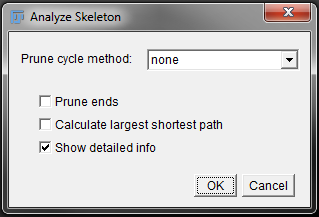
\includegraphics[width=0.4\textwidth]{mod3/figures/analyze-skeleton-dialog.png}%
		}
		\medskip
		\captionof{figure}{Analyze skeleton window.}\label{fig:analyze-skeleton-dialog}
		\end{center}
	\end{minipage}
	
	\item Three windows show up: Detailed information about each branch, summary results with branch statistics, and an image showing the skeleton with branch points and end points in different colors. You can try out different prune methods and compare the results. 
	
	\end{enumerate}
\end{taskbox}

\subsection{Watershed transform}
Watershed segmentation is used to separate touching objects, i.e. they appear as a single object in the binary image. The algorithm first calculates an Euclidean distance map (Fig. \ref{fig:distance-transform}), where the distance of each pixel to the nearest foreground pixel is calculated. The remaining black objects (peaks after the distance transform, centers of the original binary objects) are then dilated until the edge of the original object is found or the edge touches a region of another dilating object. This approach works best if the objects are 'round-ish' and have small overlap.

\begin{figure}[ht]
	\centering
		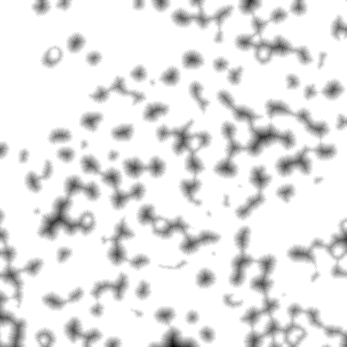
\includegraphics[width=0.60\textwidth]{mod3/figures/distance-transform.png}
	\caption{Distance transform}
	\label{fig:distance-transform}
\end{figure}

\begin{taskbox}{Watershed transform}
\begin{enumerate}
	\item Open the image bunch-of-nuclei.tif in /data/chapter4. Use the gauss-filter and thresholding to generate a binary image with the nuclei detected. Duplicate. 
	\item Use \texttt{[Process > Binary > Watershed]} on the binary image. Observe where the algorithm splits objects.
	\end{enumerate}
\end{taskbox}

\section{Analyzing objects}

Fiji has a very powerful method to obtain measurements from segmented objects which is called 'Analyze Particles' (Fig. \ref{fig:analyze-particles-dialog}). The windows allows you to select detected objects by size and by circularity, excluding objects at the edges of the image and produces several result outputs. It can add detected objects as individual ROIs to the ROI manager and perform calculations by performing the 'Measure' method on each detected object.

\begin{figure}[!ht]
	\centering
		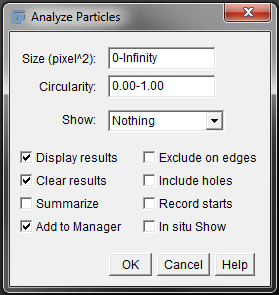
\includegraphics[width=0.40\textwidth]{mod3/figures/analyze-particles-dialog.png}
	\caption{Analyze Particles Window}
	\label{fig:analyze-particles-dialog}
\end{figure}

\begin{taskbox}{Analyze Particles}
\begin{enumerate}
	\item Open the image bunch-of-nuclei.tif in /mod3/data and use a sequence of filtering, thresholding and binary operations to identify the nuclei. Remember that this image does not provide an easy perfect result on purpose!
	\item Set the measurements you want to perform \texttt{[Analyze > Set Measurements...]}. For this example, we want at least measure the area and the mean gray value. 
	\item Perform \texttt{[Analyze > Analyze Particles...]}. Do not select objects by size or circularity, show the outlines and tick 'Display results', 'Clear results', 'Add to Manager' and 'Summarize'.
	\item Several windows should show up. A summary report indicating the number of detected objects, and several average statistics; A results window showing the selected measurements for each detected object; an outline image indicating the object number for each object; the ROI Manager with each object as an individual ROI. Why is the mean intensity value $255$ for each object? The measurement was performed on the thresholded binary image. While thresholding does not change the shape of an object, the intensity values are obviously not maintained. In order to perform the measurements on the original image, Redirect the measurements to the original image in 'Set Measurements...'.
	\item Explore the functions of the particle-analyzer method and try to select objects in a way that only small/large or round objects are measured.
	\end{enumerate}
\end{taskbox}

\subsection{Working with Plugins: Trainable Segmentation}
Machine learning methods can be used to let the computer learn what you think as object and background. Fiji has a Trainable Weka Segmentation plugin. Using this plugin, you can manually mark pixels as signal or background and let the plugin 'learn' the differences between these two classes of pixels. To achieve this differences learning, the plugin uses many features of the pixels to come up with a model that categorizes the pixels into classes. 

\begin{taskbox}{Trainable Weka Segmentation}
\begin{enumerate}
	\item Open the image tissue-adipocytes.tif in /mod3/data if it is not already open.
	\item Go to \texttt{[Plugins > Segmentation > Trainable Weka Segmentation]}. A window pops up that shows the image and several buttons (Fig. \ref{fig:weka-segmentation-window}).
	
	\begin{minipage}[t]{\linewidth}
		\begin{center}
		\adjustbox{valign=t}{%
			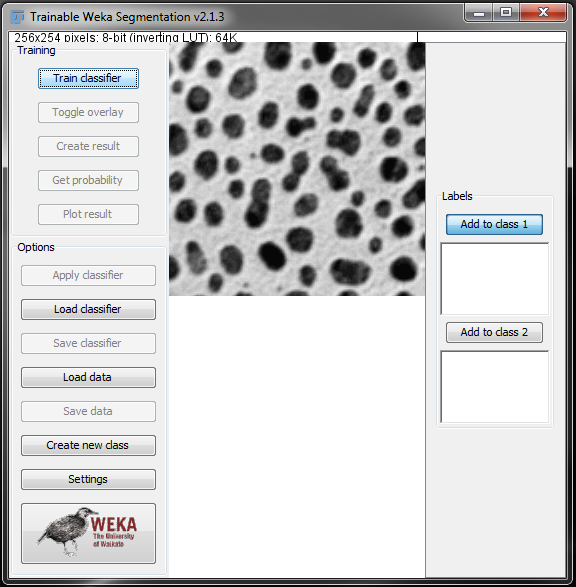
\includegraphics[width=0.8\textwidth]{mod3/figures/weka-segmentation-window.png}%
		}
		\medskip
		\captionof{figure}{Trainable segmentation window.}\label{fig:weka-segmentation-window}
		\end{center}
	\end{minipage}
	
	\item Use the freehand line tool and draw on an image object you want to detect. Add this selection to class 1. Repeat this step and then add two background selections to class 2. 
	\item Click on 'Train classifier'. You should now see what the method thinks is background and foreground. If you click on 'Create result' a two color image is generated that can easily be converted into a binary image.
	
\end{enumerate}

You have now seen the most basic usage of this plugin. For example, you could use more than two classes or apply a learned classifier to more than one file.
\end{taskbox}
